\section{SVM}

\begin{frame}
	
  \centerline{\textbf{\Huge{SVM}}}
           
	\begin{figure}[ht]
	\centering
	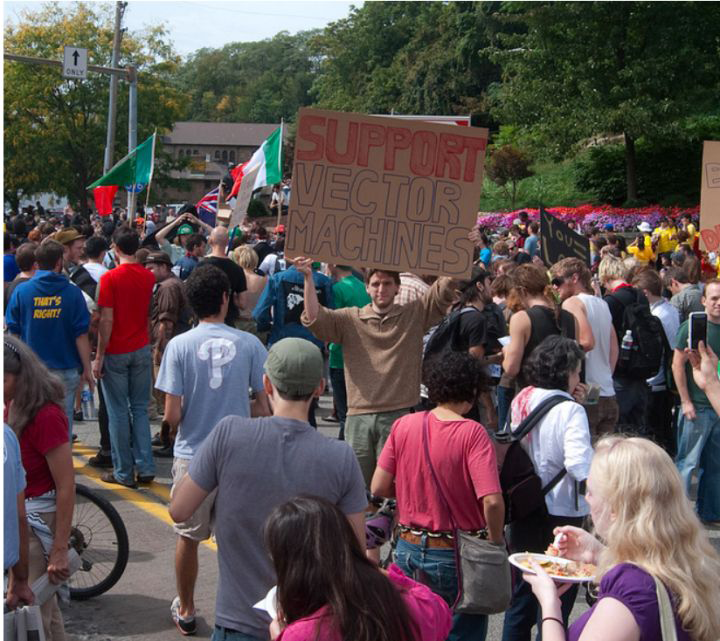
\includegraphics[width=0.5\linewidth]{partition/img/svm_0.png}  
%	\caption{this is a figure demo}
%	\label{fig:label}
	\end{figure}

\end{frame} 

\begin{frame} 
\frametitle{支持向量机}  
\begin{columns}

\column{.5\textwidth}
	\begin{itemize}
		\item SVM, 俗称支持向量机,为一种supervised learning算法,属于classification的范畴。
		\item 在数据挖掘的应用中,与unsupervised的Clustering相对应和区别。
		\item 广泛应用于机器学习(Machine Learning), 计算机视觉(Computer Vision) 和数据挖掘(Data Mining)当中。	
	\end{itemize}

\column{.5\textwidth}
	\begin{figure}[ht]
	\centering
	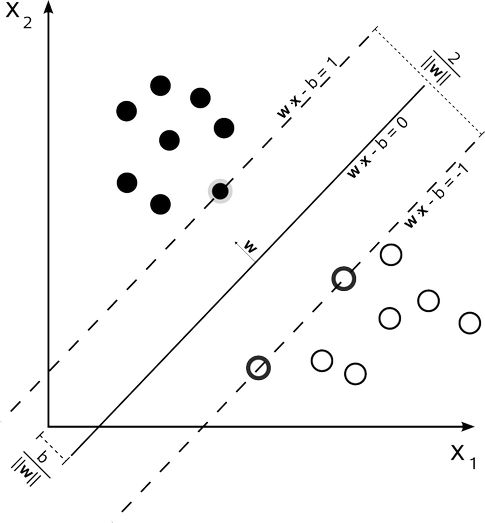
\includegraphics[width=\linewidth]{partition/img/svm_1.jpg}  
%	\caption{this is a figure demo}
%	\label{fig:label}
	\end{figure}


\end{columns}
\end{frame} 

\begin{frame}
\frametitle{一个游戏}	
现在桌子上有两种颜色的球,现在要把他们分开。
           
	\begin{figure}[ht]
	\centering
	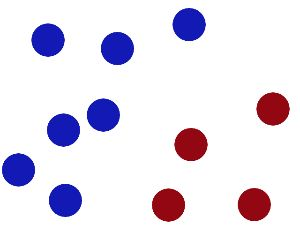
\includegraphics[width=0.5\linewidth]{partition/img/svm_2.jpg}  
%	\caption{this is a figure demo}
%	\label{fig:label}
	\end{figure}

\end{frame} 

\begin{frame}
\frametitle{一个游戏}	
我们把一根棍子放在中间,看上去干得不错。
           
	\begin{figure}[ht]
	\centering
	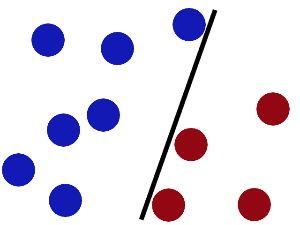
\includegraphics[width=0.5\linewidth]{partition/img/svm_3.jpg}  
%	\caption{this is a figure demo}
%	\label{fig:label}
	\end{figure}

\end{frame} 

\begin{frame}
\frametitle{一个游戏}	
有些人又往桌子上放了一些球,大部分都分对了,但是出现了一个错分的。
           
	\begin{figure}[ht]
	\centering
	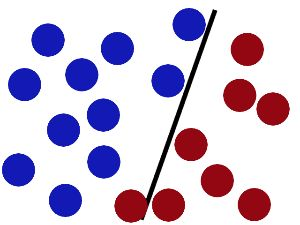
\includegraphics[width=0.5\linewidth]{partition/img/svm_4.jpg}  
%	\caption{this is a figure demo}
%	\label{fig:label}
	\end{figure}

\end{frame} 

\begin{frame}
\frametitle{一个游戏}	
SVM就是试图把棍放在最佳位置,好让在棍的两边有尽可能大的间隙。
           
	\begin{figure}[ht]
	\centering
	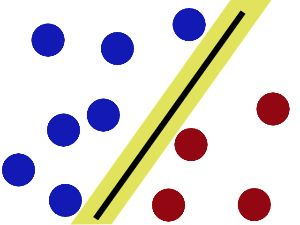
\includegraphics[width=0.5\linewidth]{partition/img/svm_5.jpg}  
%	\caption{this is a figure demo}
%	\label{fig:label}
	\end{figure}

\end{frame} 

\begin{frame}
\frametitle{一个游戏}	
现在即使放了更多的球,棍仍然是一个好的分界线
           
	\begin{figure}[ht]
	\centering
	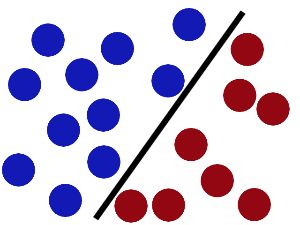
\includegraphics[width=0.5\linewidth]{partition/img/svm_6.jpg}  
%	\caption{this is a figure demo}
%	\label{fig:label}
	\end{figure}

\end{frame} 

\begin{frame}
\frametitle{一个游戏}	
 我们已经学会了一个trick,然后,在SVM 工具箱中有另一个更加重要的 trick,于是又有一个新的挑战。
           
	\begin{figure}[ht]
	\centering
	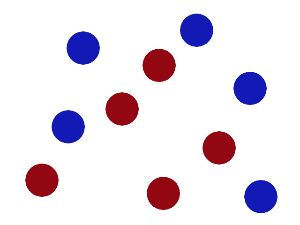
\includegraphics[width=0.5\linewidth]{partition/img/svm_7.jpg}  
%	\caption{this is a figure demo}
%	\label{fig:label}
	\end{figure}

\end{frame} 

\begin{frame}
\frametitle{一个游戏}	
现在,没有棍可以很好地分开两种球了,现在怎么办呢?我们可以一拍桌子,球飞到空中。然后,抓起一张纸,插到了两种球的中间。
           
	\begin{figure}[ht]
	\centering
	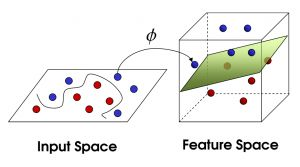
\includegraphics[width=0.5\linewidth]{partition/img/svm_8.jpg}  
%	\caption{this is a figure demo}
%	\label{fig:label}
	\end{figure}

\end{frame} 

\begin{frame}
\frametitle{一个游戏}	
现在,这些球看起来像是被一条曲线分开了。
           
	\begin{figure}[ht]
	\centering
	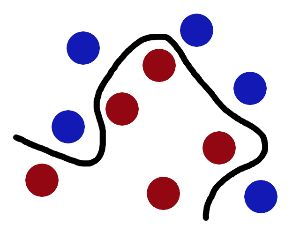
\includegraphics[width=0.5\linewidth]{partition/img/svm_9.jpg}  
%	\caption{this is a figure demo}
%	\label{fig:label}
	\end{figure}

\end{frame} 


\begin{frame}
\frametitle{怎么求解SVM?}
给定训练样本集$D = \{(x_1,y_1),(x_2,y_2),\dots,(x_m,y_m)\}$
 如果可以用一个线性超平面将其完全分开,那么这个超平面可以表示为:
\[\boldsymbol{w}^T\boldsymbol{x}+b=0\]
 其中$\boldsymbol{w}$决定了平面的方向,而b决定了平面与原点之间的距离。
           
	\begin{figure}[ht]
	\centering
	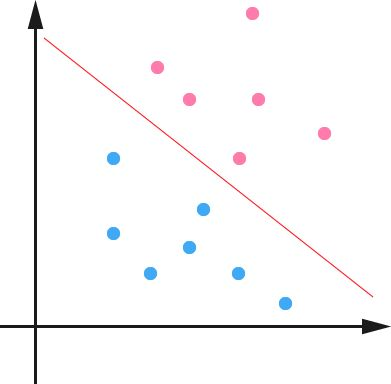
\includegraphics[width=0.5\linewidth]{partition/img/svm_10.jpg}  
%	\caption{this is a figure demo}
%	\label{fig:label}
	\end{figure}

\end{frame} 

\begin{frame}
\frametitle{间隔与支持向量}
空间中任意点$\boldsymbol{x}$实际上是一个向量,其到超平面的距离为:
\[r=\frac{\boldsymbol{w}^T\boldsymbol{x}+b}{\|\boldsymbol{w}\|}\]
	\begin{figure}[ht]
	\centering
	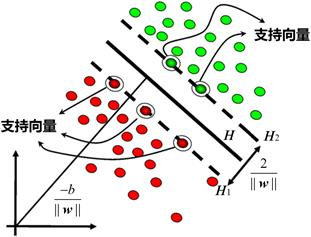
\includegraphics[width=0.5\linewidth]{partition/img/svm_11.jpg}  
%	\caption{this is a figure demo}
%	\label{fig:label}
	\end{figure}
\end{frame}

\begin{frame}
\frametitle{间隔与支持向量}
那么,如果这个超平面分类成功,我们令
\[\begin{cases}
\boldsymbol{w}^T\boldsymbol{x}+b\geq+1,\ y_i=+1\ ;\\
\boldsymbol{w}^T\boldsymbol{x}+b\leq-1,\ y_i=-1\ .
\end{cases} \]

	\begin{figure}[ht]
	\centering
	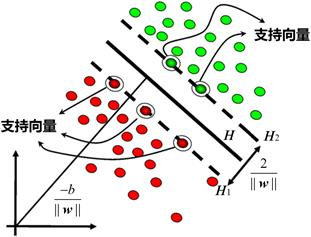
\includegraphics[width=0.5\linewidth]{partition/img/svm_11.jpg}  
%	\caption{this is a figure demo}
%	\label{fig:label}
	\end{figure}
\end{frame}

\begin{frame}
\frametitle{间隔与支持向量}

这样,那些使等号成立的点,也即距离超平面最近的点称作支持向量 (support vector),两个类到超平面距离之和也即两类之间的间隔 (margin) 是
\[
\gamma=\frac{2}{\|\boldsymbol{w}\|}
\]
训练支持向量机,实际上是希望找到具有最大间隔的划分超平面,即训练目标是在满足分类任务的情况下最大化$\gamma$,也即最大化$\|\boldsymbol{w}\|^{-1}$,也即最小化$\|\boldsymbol{w}\|^2$。
SVM的基本型就是:

\begin{gather*}
\min\limits_{\boldsymbol{w},b} \frac{1}{2}\|\boldsymbol{w}\|^2\\
s.t.\ y_i(\boldsymbol{w}^T\boldsymbol{x}_i+b)\geq1,\ i=1,2,\dots,m
\end{gather*}

%	\begin{figure}[ht]
%	\centering
%	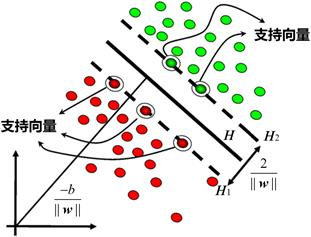
\includegraphics[width=0.3\linewidth]{partition/img/svm_11.jpg}  
%%	\caption{this is a figure demo}
%%	\label{fig:label}
%	\end{figure}
\end{frame}

\begin{frame}
\frametitle{对偶问题}
SVM的基本型是一个凸二次规划问题,可用现成的优化计算进行求解,求解的参数主要是$\boldsymbol{w}$ 和$b$。但我们可以有更高效的算法。使用拉格朗日乘子法可得到对偶问题,具体来说,对每条约束添加拉格朗日乘子$\alpha_i \ge0$,则该函数的拉格朗日函数可写为:
\[
\mathcal{L}(\boldsymbol{w},b,\boldsymbol{\alpha})=\frac{1}{2}\|\boldsymbol{w}\|^2-\sum_{i=1}^n\alpha_i \left(y_i(\boldsymbol{w}^T\boldsymbol{x_i}+b)-1\right)
\]
其中$\boldsymbol{\alpha} = (\alpha_1;\alpha_2;\dots;\alpha_m)$.令$\mathcal{L}(\boldsymbol{w},b,\boldsymbol{\alpha})$对$\boldsymbol{w}$和$b$的偏导为零可得
\begin{align*}
\boldsymbol{w} &= \sum_{i=1}^n\alpha_i y_i \boldsymbol{x}_i\ ,\\
0&=\sum_{i=1}^m\alpha_iyi\ .
\end{align*}

\end{frame}


\begin{frame}

\frametitle{对偶问题}

将$\boldsymbol{w}$结果代入,即可将$\mathcal{L}(\boldsymbol{w},b,\boldsymbol{\alpha})$中的$\boldsymbol{w}$和$b$消去,再考虑第二个式子的约束,得到对偶问题:

\begin{align*}
 \max_\alpha &\sum_{i=1}^m\alpha_i – \frac{1}{2}\sum_{i=1}^m\sum_{j=1}^m\alpha_i\alpha_jy_iy_j\boldsymbol{x_i}^T\boldsymbol{x_j} \\ 
 s.t.,&\sum_{i=1}^m\alpha_iy_i = 0 \\
  &\alpha_i\geq 0, i=1,2,\ldots,m
 \end{align*}

解出$\boldsymbol{\alpha}$后,求出$\boldsymbol{w}$与$b$即可得到模型

\begin{align*}
f(x)&=\boldsymbol{w}^T\boldsymbol{x}+b\\
&=\sum_{i=1}^m\alpha_i y_i \boldsymbol{x_i}^T\boldsymbol{x}+b 
= \sum_{i=1}^m\alpha_i y_i \langle\boldsymbol{x_i, x}\rangle + b
\end{align*}

\end{frame}


\begin{frame}

\frametitle{对偶问题}

上述过程需要满足KKT(Karush-Kuhn-Tucker)条件,即要求:
\[ 
\begin{cases}
\alpha_i \geq0\ ; \\
y_if(\boldsymbol{x_i})-1\geq 0\ ;\\
\alpha_i(y_if(\boldsymbol{x_i}-1)=0\ .
\end{cases} 
\]

\end{frame}


\begin{frame}

\frametitle{核函数}

    我们上面得到的SVM只能处理线性的问题,并不能处理非线性的问题,如果需要解决这种问题,那么其实就需要将低维数据转化到高维空间,从而找到一个超平面将其分割开来。简单的说,我们需要找到一个函数,可以将我们的原始特征通过这个函数进行映射。\\
    我们前面得到的函数形式是:
 \[
 f(x)= \sum_{i=1}^m\alpha_i y_i \langle\boldsymbol{x_i, x}\rangle + b
 \]
 则映射过后变成:  
  \[
 f(x)= \sum_{i=1}^m\alpha_i y_i \langle\boldsymbol{\phi(x_i),\phi(x)}\rangle + b
 \]

\end{frame}


\begin{frame}

\frametitle{核函数}

同样的求解形式:
\begin{align*}
 \max_\alpha &\sum_{i=1}^m\alpha_i – \frac{1}{2}\sum_{i=1}^m\sum_{j=1}^m\alpha_i\alpha_jy_iy_j\langle\boldsymbol{\phi(x_i)},\boldsymbol{\phi(x_j)}\rangle \\ 
 s.t.,&\sum_{i=1}^m\alpha_iy_i = 0 \\
  &\alpha_i\geq 0, i=1,2,\ldots,m
 \end{align*}

 很直接的想法是,我先通过$\phi(x)$将x映射到高维空间,然后再做内积运算,但在这种运算方式并不推荐,二维空间如果选择一阶二阶的组合就有5个维度,如果将维数和组合复杂度提高的话,那么映射的空间维度就会爆炸性的增长,从而为计算带来了很大的困难。那么此时我们就可以用核函数的方法来解决这类问题.
\end{frame}


\begin{frame}

\frametitle{核函数}

可以设想这样的一个函数:
\[
\kappa(\boldsymbol{x_i,x_j})=\langle\boldsymbol{\phi(x_i),\phi(x_j)}\rangle = \phi(\boldsymbol{x_i})^T\phi(\boldsymbol{x_j})
\]

即$\boldsymbol{x_i}$和$\boldsymbol{x_j}$在特征空间的内积等于他们在原始样本空间中通过函数$\kappa(\cdot,\cdot)$计算的结果.有了这样的函数,我们就不必去计算高维甚至无穷维特征空间中的内积。于是求解式可以重写为:
\begin{align*}
 \max_\alpha &\sum_{i=1}^m\alpha_i – \frac{1}{2}\sum_{i=1}^m\sum_{j=1}^m\alpha_i\alpha_jy_iy_j\kappa(\boldsymbol{x_i,x_j}) \\ 
 s.t.,&\sum_{i=1}^m\alpha_iy_i = 0 \\
  &\alpha_i\geq 0, i=1,2,\ldots,m
 \end{align*}
\end{frame}


\begin{frame}

\frametitle{核函数}

求解后即可得到:
\begin{align*}
f(x)&=\boldsymbol{w}^T\phi(\boldsymbol{x})+b\\
&=\sum_{i=1}^m\alpha_i y_i \phi(\boldsymbol{x_i})^T\phi(\boldsymbol{x})+b\\
&= \sum_{i=1}^m\alpha_i y_i \kappa(\boldsymbol{x_i, x}) + b
\end{align*}
\end{frame}



\begin{frame}

\frametitle{软间隔}
 在很多实际问题,由于存在各种噪音,所以现实生活中的分类可能并不能直接通过一个超平面将其完全分隔开来,即使能完全分隔,但得到的超平面也不一定是最佳的,如图中的情况。所以,我们需要对某些样本有一定的容忍度,允许他们跑到分隔区域中,那么原来的约束条件需要进行变化
 \begin{figure}[ht]
	\centering
	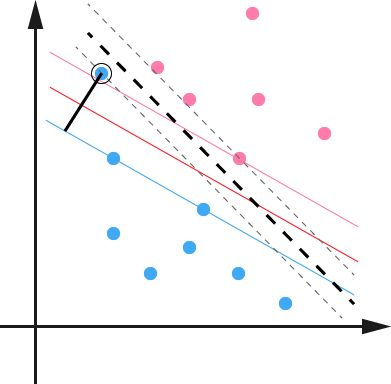
\includegraphics[width=0.5\linewidth]{partition/img/svm_12.jpg}  
%	\caption{this is a figure demo}
%	\label{fig:label}
	\end{figure}
 
\end{frame}


\begin{frame}

\frametitle{软间隔}
\[
y_i(w^Tx_i+b)\geq 1-\xi_i, \quad i=1,\ldots,n
\]
其中C是一个预先设定的值,很明显,当C无穷大时,就代表了 $\xi_i=0$ ,即是之前的那种情况。那么优化问题完整的写出来:

\begin{align*}
\min & \frac{1}{2}\|w\|^2 + C\sum_{i=1}^n\xi_i \\
 s.t., & y_i(w^Tx_i+b)\geq 1-\xi_i, i=1,\ldots,n \\
& \xi_i \geq 0, i=1,\ldots,n 
\end{align*}


\end{frame}


\begin{frame}
\frametitle{软间隔}

用之前的方法可得:
\[
\mathcal{L}(w,b,\xi,\alpha,r)=\frac{1}{2}\|w\|^2 + C\sum_{i=1}^n\xi_i – \sum_{i=1}^n\alpha_i \left(y_i(w^Tx_i+b)-1+\xi_i\right) – \sum_{i=1}^n r_i\xi_i
\]

求导可得:

\begin{align*}
\frac{\partial \mathcal{L}}{\partial w}=0 &\Rightarrow w=\sum_{i=1}^n \alpha_i y_i x_i \\
\frac{\partial \mathcal{L}}{\partial b} = 0 &\Rightarrow \sum_{i=1}^n \alpha_i y_i = 0 \\
\frac{\partial \mathcal{L}}{\partial \xi_i} = 0 &\Rightarrow C-\alpha_i-r_i=0, \quad i=1,\ldots,n 
\end{align*}

\end{frame}


\begin{frame}
\frametitle{软间隔}

带回原式,可以看到目标函数并没有发生变化,但约束条件变了:

\begin{align*}
\max_\alpha &\sum_{i=1}^n\alpha_i – \frac{1}{2}\sum_{i,j=1}^n\alpha_i\alpha_jy_iy_j\langle x_i,x_j\rangle \\
s.t., &0\leq \alpha_i\leq C, i=1,\ldots,n \\
&\sum_{i=1}^n\alpha_iy_i = 0
\end{align*}
那么对于任意样本$(x_i,y_i)$ ,总有 $a_i=0$ 或$ y_if(x_i) = 1-\xi_i$  ,若 $a_i=0$ ,则样本不会对$ f(x)$ 有影响;若$ a_i>0$ ,则必有$ y_if(x_i) = 1-\xi_i$ ,即该样本就是支持向量。若 $a_i<C$ ,则有 $\xi_i=0$ ,即该样本落在间隔界线上,若 $a_i=C$ ,则样本落在间隔内部。
\end{frame}